%%
%% This is file `sample-authordraft.tex',
%% generated with the docstrip utility.
%%
%% The original source files were:
%%
%% samples.dtx  (with options: `authordraft')
%% 
%% IMPORTANT NOTICE:
%% 
%% For the copyright see the source file.
%% 
%% Any modified versions of this file must be renamed
%% with new filenames distinct from sample-authordraft.tex.
%% 
%% For distribution of the original source see the terms
%% for copying and modification in the file samples.dtx.
%% 
%% This generated file may be distributed as long as the
%% original source files, as listed above, are part of the
%% same distribution. (The sources need not necessarily be
%% in the same archive or directory.)
%%
%% The first command in your LaTeX source must be the \documentclass command.
\documentclass[sigconf,authordraft]{acmart}
%% NOTE that a single column version may be required for 
%% submission and peer review. This can be done by changing
%% the \doucmentclass[...]{acmart} in this template to 
%% \documentclass[manuscript,screen,review]{acmart}
%% To ensure 100% compatibility, please check the white list of
%% approved LaTeX packages to be used with the Master Article Template at
%% https://www.acm.org/publications/taps/whitelist-of-latex-packages 
%% before creating your document. The white list page provides 
%% information on how to submit additional LaTeX packages for 
%% review and adoption.
%% Fonts used in the template cannot be substituted; margin 
%% adjustments are not allowed.
%%
%% \BibTeX command to typeset BibTeX logo in the docs
\AtBeginDocument{%
  \providecommand\BibTeX{{%
    \normalfont B\kern-0.5em{\scshape i\kern-0.25em b}\kern-0.8em\TeX}}}

%% Rights management information.  This information is sent to you
%% when you complete the rights form.  These commands have SAMPLE
%% values in them; it is your responsibility as an author to replace
%% the commands and values with those provided to you when you
%% complete the rights form.
\setcopyright{acmcopyright}
\copyrightyear{2021}
\acmYear{2021}
\acmDOI{10.1145/1122445.1122456}

%%
%% Submission ID.
%% Use this when submitting an article to a sponsored event. You'll
%% receive a unique submission ID from the organizers
%% of the event, and this ID should be used as the parameter to this command.
%%\acmSubmissionID{123-A56-BU3}

%%
%% The majority of ACM publications use numbered citations and
%% references.  The command \citestyle{authoryear} switches to the
%% "author year" style.
%%
%% If you are preparing content for an event
%% sponsored by ACM SIGGRAPH, you must use the "author year" style of
%% citations and references.
%% Uncommenting
%% the next command will enable that style.
%%\citestyle{acmauthoryear}

%%
%% end of the preamble, start of the body of the document source.
\begin{document}

%%
%% The "title" command has an optional parameter,
%% allowing the author to define a "short title" to be used in page headers.
\title{Methods Included: Standardizing Computational Reuse and Portability
with the Common Workflow Language}

%%
%% The "author" command and its associated commands are used to define
%% the authors and their affiliations.
%% Of note is the shared affiliation of the first two authors, and the
%% "authornote" and "authornotemark" commands
%% used to denote shared contribution to the research.
\author{Michael R. Crusoe}
\orcid{0000-0002-2961-9670}
\affiliation{%
  \institution{VU Amsterdam}
  \streetaddress{De Boelelaan 1111}
  \city{Amsterdam}
  \country{Netherlads}
  \postcode{1081 HV}
}
\affiliation{%
  \institution{CWL Project @ Software Freedom Conservancy}
  \streetaddress{137 MONTAGUE ST STE 380}
  \city{Brooklyn}
  \state{NY}
  \country{USA}
  \postcode{11201-3548}
}
\email{mrc@commonwl.org}

\author{Sanne Abeln}
\orcid{0000-0002-2779-7174}
\affiliation{%
  \institution{VU Amsterdam}
  \streetaddress{De Boelelaan 1111}
  \city{Amsterdam}
  \country{Netherlads}
  \postcode{1081 HV}
}
\email{s.abeln@vu.nl}

\author{Alexandru Iosup}
\orcid{0000-0001-8030-9398}
\affiliation{%
  \institution{VU Amsterdam}
  \streetaddress{De Boelelaan 1111}
  \city{Amsterdam}
  \country{Netherlads}
  \postcode{1081 HV}
}
\email{a.iosup@vu.nl}

\author{Peter Amstutz}
\orcid{0000-0003-3566-7705}
\affiliation{%
  \institution{Curii, Inc.}
  \streetaddress{212 Elm St. 3rd Floor}
  \city{Sommerville}
  \state{MA}
  \country{USA}
  \postcode{02144-2959}
}
\email{peter.amstutz@curii.com}

\author{John Chilton}
\orcid{0000-0002-6794-0756}
\affiliation{%
  \institution{Pennsylvania State University / Galaxy Project}
  \city{State College}
  \state{PA}
  \country{USA}
  \postcode{16801}
}
\email{jmchilton@gmail.com}

\author{Nebojša Tijanić}
\orcid{0000-0001-8316-4067}
\affiliation{%
  \institution{Totient}
  \streetaddress{1 Alewife Center Suite 120}
  \city{Cambridge}
  \state{MA}
  \country{USA}
  \postcode{02140}
}
\email{boysha@gmail.com}

\author{Hervé Ménager}
\orcid{0000-0002-7552-1009}
\affiliation{%
  \institution{Institut Pasteur}
  \streetaddress{25-28 Rue du Dr Roux}
  \city{Paris}
  \country{France}
  \postcode{75015}
}
\email{herve.menager@pasteur.fr}

\author{Stian Soiland-Reyes}
\orcid{0000-0001-9842-9718}
\affiliation{%
  \institution{Department of Computer Science, The University of Manchester}
  \city{Manchester}
  \country{UK}
}
\affiliation{%
  \institution{Informatics Institute, University of Netherlands}
  \country{Netherlands}
}
\email{soiland-reyes@manchester.ac.uk}

\author{Carole Goble}
\orcid{0000-0003-1219-2137}
\affiliation{%
  \institution{Department of Computer Science, The University of Manchester}
  \city{Manchester}
  \country{UK}
}
\email{carole.goble@manchester.ac.uk}

\author{The CWL Community}

%%
%% By default, the full list of authors will be used in the page
%% headers. Often, this list is too long, and will overlap
%% other information printed in the page headers. This command allows
%% the author to define a more concise list
%% of authors' names for this purpose.
\renewcommand{\shortauthors}{Crusoe et al.}

%%
%% The abstract is a short summary of the work to be presented in the
%% article.
\begin{abstract}
  TODO
\end{abstract}

%%
%% The code below is generated by the tool at http://dl.acm.org/ccs.cfm.
%% Please copy and paste the code instead of the example below.
%%
\begin{CCSXML}
<ccs2012>
   <concept>
       <concept_id>10010147.10010919</concept_id>
       <concept_desc>Computing methodologies~Distributed computing methodologies</concept_desc>
       <concept_significance>500</concept_significance>
       </concept>
   <concept>
       <concept_id>10002944.10011122.10003459</concept_id>
       <concept_desc>General and reference~Computing standards, RFCs and guidelines</concept_desc>
       <concept_significance>500</concept_significance>
       </concept>
   <concept>
       <concept_id>10010405.10010432.10010435</concept_id>
       <concept_desc>Applied computing~Astronomy</concept_desc>
       <concept_significance>500</concept_significance>
       </concept>
   <concept>
       <concept_id>10010405.10010432.10010437</concept_id>
       <concept_desc>Applied computing~Earth and atmospheric sciences</concept_desc>
       <concept_significance>300</concept_significance>
       </concept>
   <concept>
       <concept_id>10010405.10010406.10011731</concept_id>
       <concept_desc>Applied computing~Enterprise interoperability</concept_desc>
       <concept_significance>300</concept_significance>
       </concept>
   <concept>
       <concept_id>10010405.10010406.10010431</concept_id>
       <concept_desc>Applied computing~Enterprise computing infrastructures</concept_desc>
       <concept_significance>300</concept_significance>
       </concept>
   <concept>
       <concept_id>10010405.10010444</concept_id>
       <concept_desc>Applied computing~Life and medical sciences</concept_desc>
       <concept_significance>300</concept_significance>
       </concept>
   <concept>
       <concept_id>10010405.10010444.10010450</concept_id>
       <concept_desc>Applied computing~Bioinformatics</concept_desc>
       <concept_significance>500</concept_significance>
       </concept>
   <concept>
       <concept_id>10010405.10010444.10010935.10010454</concept_id>
       <concept_desc>Applied computing~Transcriptomics</concept_desc>
       <concept_significance>500</concept_significance>
       </concept>
   <concept>
       <concept_id>10010405.10010444.10010935.10010451.10010097</concept_id>
       <concept_desc>Applied computing~Computational proteomics</concept_desc>
       <concept_significance>500</concept_significance>
       </concept>
   <concept>
       <concept_id>10010405.10010444.10010935.10010094</concept_id>
       <concept_desc>Applied computing~Population genetics</concept_desc>
       <concept_significance>300</concept_significance>
       </concept>
   <concept>
       <concept_id>10010405.10010444.10010095</concept_id>
       <concept_desc>Applied computing~Systems biology</concept_desc>
       <concept_significance>300</concept_significance>
       </concept>
   <concept>
       <concept_id>10010405.10010444.10010087</concept_id>
       <concept_desc>Applied computing~Computational biology</concept_desc>
       <concept_significance>300</concept_significance>
       </concept>
   <concept>
       <concept_id>10010405.10010444.10010087.10010097</concept_id>
       <concept_desc>Applied computing~Computational proteomics</concept_desc>
       <concept_significance>500</concept_significance>
       </concept>
   <concept>
       <concept_id>10010405.10010444.10010087.10010934</concept_id>
       <concept_desc>Applied computing~Computational genomics</concept_desc>
       <concept_significance>500</concept_significance>
       </concept>
   <concept>
       <concept_id>10010405.10010444.10010087.10010096</concept_id>
       <concept_desc>Applied computing~Imaging</concept_desc>
       <concept_significance>500</concept_significance>
       </concept>
   <concept>
       <concept_id>10010405.10010444.10010087.10010090</concept_id>
       <concept_desc>Applied computing~Computational transcriptomics</concept_desc>
       <concept_significance>500</concept_significance>
       </concept>
 </ccs2012>
\end{CCSXML}

\ccsdesc[500]{Computing methodologies~Distributed computing methodologies}
\ccsdesc[500]{General and reference~Computing standards, RFCs and guidelines}
\ccsdesc[500]{Applied computing~Astronomy}
\ccsdesc[300]{Applied computing~Earth and atmospheric sciences}
\ccsdesc[300]{Applied computing~Enterprise interoperability}
\ccsdesc[300]{Applied computing~Enterprise computing infrastructures}
\ccsdesc[300]{Applied computing~Life and medical sciences}
\ccsdesc[500]{Applied computing~Bioinformatics}
\ccsdesc[500]{Applied computing~Transcriptomics}
\ccsdesc[500]{Applied computing~Computational proteomics}
\ccsdesc[300]{Applied computing~Population genetics}
\ccsdesc[300]{Applied computing~Systems biology}
\ccsdesc[300]{Applied computing~Computational biology}
\ccsdesc[500]{Applied computing~Computational proteomics}
\ccsdesc[500]{Applied computing~Computational genomics}
\ccsdesc[500]{Applied computing~Imaging}
\ccsdesc[500]{Applied computing~Computational transcriptomics}

%%
%% Keywords. The author(s) should pick words that accurately describe
%% the work being presented. Separate the keywords with commas.
\keywords{workflows, computational data analysis, cwl, commonwl, sciworkflows}

%%
%% This command processes the author and affiliation and title
%% information and builds the first part of the formatted document.
\maketitle

\section{Introduction}
Computational workflows are widely used in data analysis pipelines,
enabling innovation and decision-making for the modern society. But
their growing popularity is also a main cause for concern: unless we
standardize computational reuse and portability, the use of workflows
may end up hampering collaboration. How can we both enjoy the most
common benefits of computational workflows and eliminate the risks?

Workflow thinking introduces an abstraction that helps decouple
expertise in a specific domain, for example of science or of
engineering, from expertise in computing. Derived from workflow
thinking, a computational workflow describes a process for computing
where different parts of the process (the tasks) are inter-dependent -
e.g., a task can start processing only after its predecessors have
(partially) completed and where data flows between tasks. In many
domains, workflows include diverse analysis components, written in
multiple (different) computer languages, by both end-users and
third-parties. Such polylingual, and multi-party workflows are
already common or dominant in data-intensive fields like bioinformatics,
image analysis, and radio astronomy; we envision they could bring
important benefits to many other domains. To thread data through
these tools, domain experts such as bioinformaticians use specialized
command-line interfaces~\cite{seemann_ten_2013,georgeson_bionitio_2019}, and other
domains use their own customized frameworks~\cite{babuji_parsl_2019,berthold_knime_2009}.
Workflow engines also help with efficient management of the resources
used to run scientific workloads~\cite{deelman_pegasus_2015,couvares_workflow_2007}.
The workflow
approach helps compose an entire application of these command-line
analysis tools: developers build graphical or textual descriptions of
how to run these command-line tools, and scientists and engineers
connect their inputs and outputs so that the data flows through. An
example of a complex workflow problem is metagenomic analysis, a subset
is shown in Figure 1.

In practice, many research and engineering groups use workflows of
the kind described in Figure 1. However, as highlighted in a
``Technology Toolbox'' article~\cite{perkel_workflow_2019} published recently in
the journal Nature, these groups lack the ability to share and
collaborate across institutions and infrastructures without costly
manual translation. Limiting computational reuse and portability,
currently many competing workflow management systems and runners
exist, each with their syntax or method for describing workflows and
infrastructure requirements. The data flows are becoming so complex,
that their non-explicit specification in most workflow abstractions
further increases the costs to reuse and port to third-parties. We thus
identify an important problem in the broad adoption of workflow thinking
in practice: although communities want polylingual, and multi-party
workflows, adopting and managing different workflow systems is costly
and difficult. In this work, we propose to tame this complexity through
a higher-level abstraction that covers the majority of features used
in practice, and is (or can be quickly implemented) in many workflow
systems.

In the computational workflow depicted in Figure 1, practitioners
solved their problem by adopting the Common Workflow Language (CWL), an
open standard for describing command-line-tool based workflows like
theirs. We posit in this work that CWL can help solve the main problem,
and we set out to introduce the CWL standards. CWL focuses on
maintaining a separation of concerns between the description and
execution of tools and workflows. CWL supports workflow automation,
scalability, abstraction, provenance, portability, and reusability.
Last, but not least, CWL takes a principled, community-first open-source
and open-standard approach enables this result.

CWL is the product of an open and free standards-making community.
CWL began in the bioinformatics domain, but its principles are
broad. Since the ratification of the first version in 2016, the CWL
standards have seen use in other fields including hydrology~\cite{eoscpilot_ewatercycle},
radio astronomy~\cite{eoscpilot-lofar},
geo-spatial analysis~\cite{simonis_ogc_2020,goncalves_ogc_2020,landry_ogc_2020},
high energy physics~\cite{bell_web-based_2017}
in addition to the more traditional bioinformatics fields like genomics
and cancer research~\cite{kaushik_building_2019}. The many CWL contributors shaped the
standard so that it could be useful to any domain that experiences the
problem of "many tools written in many programming languages by many
parties".

CWL should also be useful beyond science, e.g., for engineering
and industrial processes. The separation of concerns CWL proposes
enables diverse projects, and should also benefit engineering and large
industrial projects. Likewise, those using software container technology
like Docker to distribute analysis tools may appreciate using only the
CWL Command Line Tool standard for providing a structured description of
how to run their tools, what data is required, and what results to
expect.

HIGHLIGHTS BOX

Toward computational reuse and portability of polylingual, and
multi-party workflows, CWL makes the following contributions:

\begin{enumerate}
\item
  {CWL is a set of standards for describing and sharing such workflows;}
\item
  {CWL is already used daily in many science and engineering domains,
  and also by multi-stakeholder teams;}
\item
  {CWL has a declarative syntax facilitating polylingual workflow tasks,
  is explicit about the runtime environment, supports software
  containers, and these together help enable portability and reuse;}
\item
  {The CWL standards provides for a separation of concerns between
  workflow authors and workflow platforms; allowing each to optimize
  without affecting the other;}
\item
  {The CWL standards supports critical workflow concepts like
  automation, scalability, abstraction, provenance, portability, and
  reusability.}
\item
  {CWL is developed around }{five principles}{~in the themes of
  community, re-use, and zero cost for participants.}
\item
  {CWL is open-source, and provides freely-available open standards via
  an open community and a Free/Open Source Software ecosystem.}
\end{enumerate}

\section{Why Workflows?}

A process, digital or otherwise, may grow to such complexity that the
authors and users of that process have difficulties in understanding its
structure, scaling the process, managing the running of the process, and
keeping track of what happened in previous enactments of the process.
Dependencies of, and within, the process may be undocumented,
obfuscated, or otherwise effectively invisible; even an extensively
documented process may be difficult to understand for lack of common
framework or vocabulary. A need to run the process more frequently or
with larger inputs may be too much for the sole entity (script or
person) that was previously running it. What was once a reasonable
manual step (run this command here and then paste the result there; call
this person for permission) may later be a bottleneck. Informal logs (if
any) quickly can become unsuitable to an organization's need to
understand what happened when by whom ("What do you mean you can't
tell me who made the decision to paint bike shed \#1001 that
color?!").

Workflow techniques aim to solve these problems by providing the
"A.S.A.P." features : Abstraction, Scaling, Automation, and Provenance~\cite{cuevas-vicenttin_scientific_2012}. Workflow constructs enable a clear abstraction about the
components, the relationships between components, and the inputs and
outputs of the components turning them into well-labeled tools with
documented expectations. This abstraction enables scaling (execution can
be parallelized and distributed), automation (the abstraction can be
used by a workflow engine to track, plan, and manage execution of
tasks), and provenance tracking (with an abstraction in place then
identifiers can be assigned to tasks, executors, inputs, outputs; all
these identifiers, timestamps, and other logs can be stored in relation
to each other to answer queries later).

Using workflow techniques, especially with digital analysis processes,
has become quite popular and does not look to be slowing down: one
platform recently celebrated its 10,000
citation \footnote{\url{https://galaxyproject.org/blog/2020-08-10k-pubs/}};
and over285 scientific workflow systems are known \footnote{\url{https://s.apache.org/existing-workflow-systems}}.
However,
prior to the adoption of the CWL standards by some systems, every
scientific workflow system was incompatible with each other, each
requiring users to express their workflows in a different way.

Local success, global \textit{un}portability. The success of workflows
is now its biggest drawback: users are locked in to a particular
vendor, project, and often a particular hardware setup; thus sharing
and re-use is hampered. Even non-academics suffer here, as the lack of
standards (or the lack of their adoption) hinders collaboration within
and between companies. Likewise for public-private partnerships and
technology transfer from public researchers.

Sharing standards-based workflow descriptions may also help to
solve a significant problem~\cite{ivie_reproducibility_2018, feitelson_repeatability_2015}: 
incomplete methods descriptions when computational analysis is involved.
Reproduction, replication, or re-use of these digital methods
requires a complete description of what computer applications were used,
how exactly they were used, and how they were connected to each other.
For precision, this description should be in an appropriate standardized
machine-readable format.

\subsection{Sidebar A: Monolingual and Polylingual workflow systems}

Workflows techniques can be implemented in many ways with varying
degrees of formalisms which tends to correlate with execution
flexibility and features. Typically the most informal techniques require
that all processing components are written in the same programming
language or are at least callable from the same programming language. On
the informal side is the do-it-yourself approach using techniques
built-in to a particular programming language: for example using the
`threading' library in Python or calling `xargs' or GNU Parallel~\cite{tange_gnu_2011} from a shell script. To gain more flexibility (while still
being based in a particular programming language) one might adopt a
third-party library that can enable remote or distributed execution
without having to re-write one's code like
`ipyparallel' \footnote{\url{https://pypi.org/project/ipyparallel/}}.
Even more structured would be the use of a programming language specific
workflow library, like Parsl~\cite{babuji_parsl_2019}, where the workflow constructs("this is a unit of processing", "here are the dependencies between
the units") are even more explicit. Here we see that Parsl is an
example of a monolingual workflow system.

Two approaches are seen to accommodate workflows where the components
are written in more than one programming language (or the components
come from third parties and the user does not want to or cannot
modify them): use of per-language add-in libraries or the use of the
POSIX command-line interface~\cite{the_austin_group_posix1-2008_2008}.
The use of per-language
add-in libraries is done by either explicit function calls or the
addition of annotations to the users functions and requires
mapping/restricting to a common cross-language data model.
Essentially all programming languages support the creation of POSIX
command line interfaces. Choosing the POSIX command-line interface
as the point of coordination means the connection between components
is done by an array of strings representing program options (including
references to data files that may contain additional configuration)
along with a string-based environment variables key-value map. This
second option has the advantage of not needing per-language
implementation at the expense of a very simple data model which leads to
a tendency for larger granularity of the units of work. As a polylingual
workflow standard, CWL uses the POSIX CLI data model.

\section{Features of the Common Workflow Language standards}

%%\begin{figure*}
%%  \centering
%% 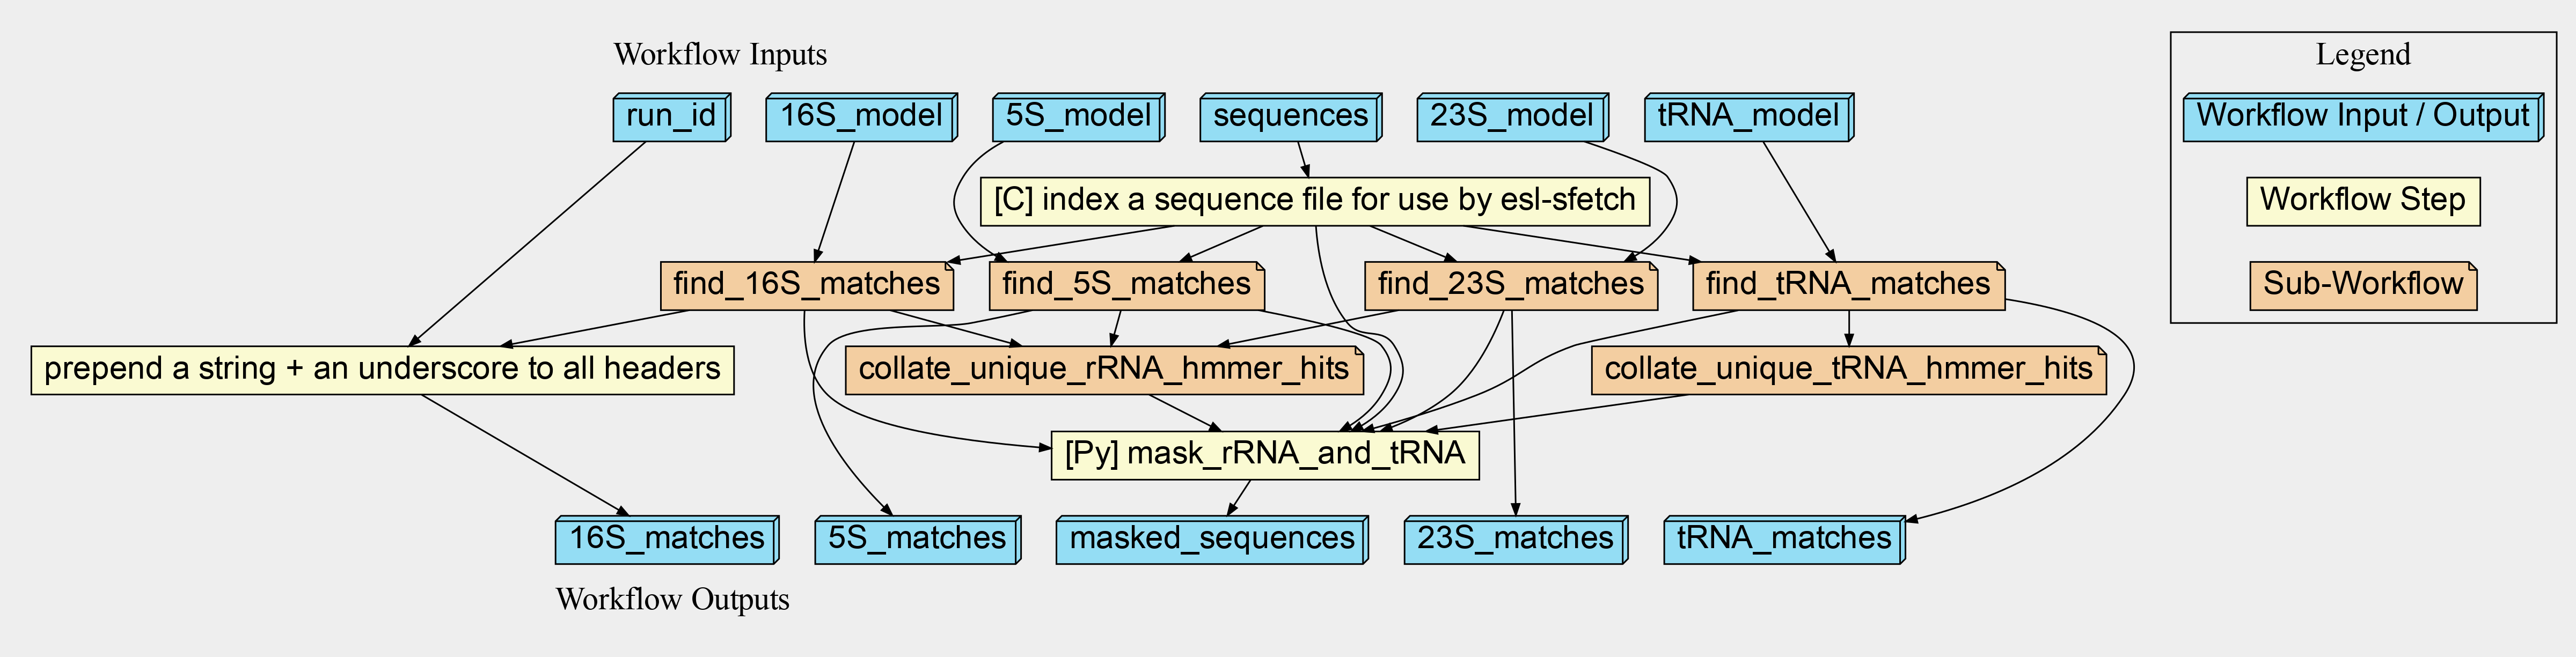
\includegraphics[width=\textwidth]{figure1.png}
%%  \caption{Excerpt \footnote{Adapted from \url{https://w3id.org/cwl/view/git/7bb76f33bf40b5cd2604001cac46f967a209c47f/workflows/rna-selector.cwl}. } from a large microbiome bioinformatics CWL workflow; this excerpt has the aim to match sequences to sequence-models. The indicators show that different steps are written in different programming languages: [Py] for Python; [C] for the C language.}
%%  \Description{TODO}
%% \end{figure*}

\begin{figure*}
  \centering
  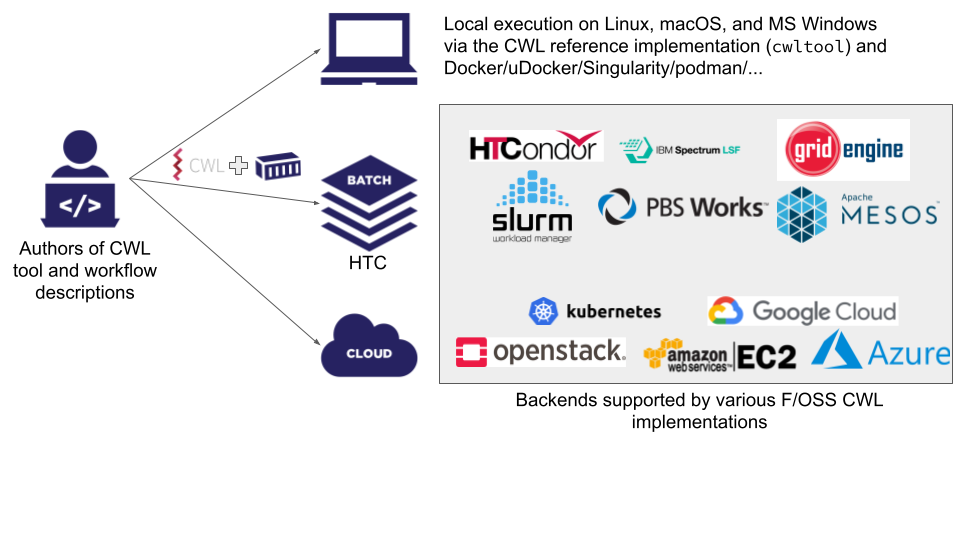
\includegraphics[width=\textwidth]{figure2.png}
  \caption{Example of CWL portability. The same workflow description runs on the scientist's own
  laptop or single machine, any batch production-environment, and any
common public or private cloud. The CWL standards enable execution
portability by being explicit about data locations. This enables
execution of CWL workflows on diverse environments as provided by
various implementations of the CWL standards: the scientist's own laptop
or single machine, any batch production-environment, and any common
public or private cloud.}
  \Description{TODO}
\end{figure*}

Each release of CWL has two
\footnote{There is a third component, the updated schema language standard “schema salad” that is used to define the syntax of CWL itself.}
main components (1) a standard for describing command line tools; (2) a
standard for describing workflows made from those the tool descriptions
defined by the first standard. The goal of the "CWL Command Line Tool
Description Standard" \footnote{\url{https://www.commonwl.org/v1.2/CommandLineTool.html}}
is to
describe how a particular command line tool works: what are the inputs
and parameters and their types; how to add the correct flags and
switches to the command line invocation; and where to find the output
files. As shown in Figure 3B, item 3, these tool descriptions can
contain hints about which software container to use; how much compute
resources are required (memory, number of CPU cores, disk space, and/or
the maximum time.

\begin{figure*}
  \centering
  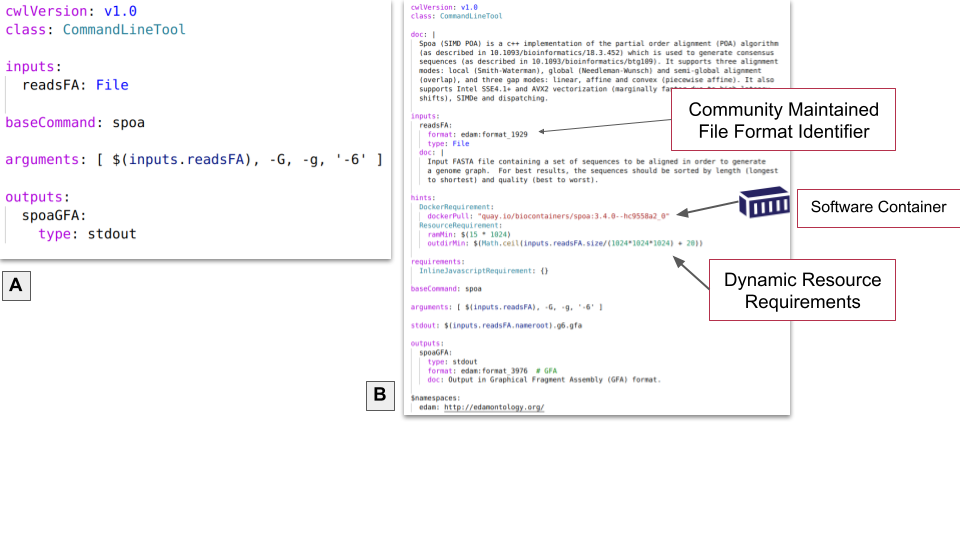
\includegraphics[width=\textwidth]{figure3.png}
  \caption{Example of CWL syntax and progressive enhancement. (A) and
(B) describe the same tool, but (B) is enhanced with additional
features: the use of file format identifiers for better documentation
and workflow connection validation; specification of a recommended
software container for more reproducible results and easier software
installation; dynamically specified resource requirements to optimize
scheduling and resource usage without manual intervention.}
  \Description{TODO}
\end{figure*}

CWL is a very explicit language, both in syntax and in its data and
execution model. Textually one would write CWL in YAML (JSON is also
acceptable, and common when converting from another format), see Figure
3A for a simple example, and Figure 3B for the same example with more
details. Each input to a tool has a name and a type; likewise for the
expected outputs. Tool description authors are encouraged to include
documentation and labels for all components (Figure 3B), this enables
automatic generation of helpful Graphical User Interfaces (GUIs) for any
given CWL description. Metadata about the tool description authors
themselves encourages attribution of their efforts.

As for the execution model: by default the CWL tool runtime environment
is explicit and starts empty, to be filled in by the CWL tool
description author \footnote{\url{https://www.commonwl.org/v1.2/CommandLineTool.html\#Runtime_environment}}.
The working directory is empty; none but a few standard environment
variables are defined; and the only files present are those that are
marked as explicit inputs. For describing the operation of very
opinionated applications, there are CWL constructs to specify that
particular environment variables must be set and the working directory
must be laid out using specific file and directory names prior to
running the tool.

Explicit runtime model enables portability by being explicit about
data locations. This enables execution of CWL workflows on diverse
environments as provided by various implementations of the CWL
standards: the local environment of the author-scientist (e.g., a single
desktop computer, laptop, or workstation), a remote batch
production-environment, and an on-demand cloud environment.

Using software container technologies like Docker, which enables
portability of the underlying analysis tools, is quite straightforward
with CWL (Figure 3B, item 2): the platform will know exactly which files
and folders to mount where, no guesswork needed. Likewise, no
changes to a CWL tool description are needed when distributed execution
is desired. All file or directory inputs must already be explicitly
defined in the CWL description; the user's workflow platform handles all
routing of data or placement of jobs.

The \textit{Common} Workflow Language standards aim to cover the common
needs of users and the common\textit{ly} implemented features of
workflow runners or platforms. To support features that are not in the
CWL standards there are extension points that permit namespaced vendor
specific features in well defined ways. If these extensions do not ~
fundamentally change how the tool should operate then they are put under
"hints" and other vendors can ignore them. However, if the vendor
extension is required to properly run the tool being described, perhaps
due to the need for some exotic custom hardware, then the extension is
put under "requirements" and other vendors know not to even accept
such a document for execution.

The "CWL Workflow Description Standard" \footnote{\url{https://www.commonwl.org/v1.2/Workflow.html}}
builds upon the CWL Command Line Tool Standard: it has the same YAML/JSON style
syntax with explicit workflow level inputs, outputs, and documentation.
Here the workflow is formed by a list of steps (made up of CWL
CommandLineTools or CWL sub-Workflows), and the workflow inputs are
connected to various inputs needed by some of the steps; the named
inputs and outputs of the steps are connected to each other as needed,
and the workflow overall outputs source themselves from select outputs
of particular workflow steps. All connections are made by identifiers,
which CWL document authors are encouraged to make meaningful names for:
"reference\_genome" instead of "input7". See Figure 3 for an
example.

This approach of modeling a workflow is the data flow paradigm;
the connectivity defines the order of execution. Parallel execution of
steps is permitted and encouraged whenever multiple steps have all of
their inputs satisfied. A "scatter" construct allows the repeated
execution of a CWL step when one, two, or more of the inputs vary but
the rest of the inputs remain constant. Starting with CWL version 1.2,
workflows can also conditionally execute a step based upon a specified
intermediate value or user provided value.

Forward compatibility of CWL documents is guaranteed as each CWL
document declares which version of the standards it was written for. A
stand alone upgrader\footnote{\url{https://pypi.org/project/cwl-upgrader/}}
can automatically upgrade CWL documents from one version to the next, and
many CWL aware platforms will internally update user submitted documents
at runtime.

\section{Open-Source, Open Standards, Open Community}

Given the numerous and diverse set of potential users, implementers,
and other stakeholders, we posit that a project like CWL requires
combined development of code, standards, and community. Indeed, these
requirements were part of the foundational design principles for CWL:

\textbf{Principle 1}: The core of the project is the community of people
who cared about the goals.

\textbf{Principle 2}: To achieve the best possible results, there should be
few, if any, barriers to participation in order to attract people with
diverse experiences and perspectives; specifically there must be no
cost to participate.

\textbf{Principle 3}: The outputs of this project should be as useful as
possible to people in whatever way they can come up with, to enable the
most good. Thus, the standards themselves must have no acquisition
price and be licensed for reuse.

\textbf{Principle 4}: The project must not favor one company or group over
another, but neither should it try to be all things to all people.

\textbf{Principle 5}: The concepts and ideas must be tested frequently,
tested and functional code is the beginning of evaluating a proposal,
not the end.

In time, the CWL project learned that this approach was a superset of
the OpenStand Principles \footnote{https://open-stand.org/about-us/principles/} , a joint ``Modern Paradigm for Standards'' promoted by the IAB, IEEE, IETF,
Internet Society, and W3C. The CWL addition to the OpenStand Principles
is to keep participation free of cost, and the explicit choice of the
Apache 2.0 license for all text, conformance tests, and the reference
implementation.

\textbf{Necessary and sufficient}: All the principles have proven to be
essential for the CWL project. For example, the free cost and open
source license (Principle 2 and 3) has enabled many implementations of
the CWL standards, several of which re-use different parts of the CWL
reference runner. Being community-first (Principle 1) has led to several
projects from participants that are outside the CWL standards
themselves.

As part of Principle 5, we developed a suite of conformance
tests for each version of the CWL standards. These publicly available
tests were critical to CWL's success: they helped prove the reference
implementation of CWL itself; they provided concrete examples to early
adopters; and they enabled the developers and users of production
implementations of the CWL standards to confirm their correctness.

\subsection{Sidebar C: CWL F/OSS Ecosystem}

\subsubsection{Free and Open Source implementations of CWL}
%%\footnote{Snapshot of TODO: fix URL}}
%% https://www.commonwl.org/\#Implementations}}

Currently the CWL community does neither test nor certify CWL
implementations, nor specific technology stacks. Platform/service
providers can confirm support for a particular technology
configuration and CWL. We recommend testing your desired technology
stack using the CWL conformance tests. In addition to the
implementations in Table 1, Galaxy~\cite{afgan_galaxy_2018}
%%\footnote{TODO: fix URLs}
%% https://github.com/common-workflow-language/galaxy/pull/47}
and Pegasus~\cite{deelman_pegasus_2015}
%%\footnote{TODO: fix URLs}
%% https://pegasus.isi.edu/documentation/manpages/pegasus-cwl-converter.html}
have in-development support for CWL as well.

\begin{table}
\begin{tabular}{cc}
\cation{Selected F/OSS workflow runners / platforms that implement the CWL standards}
\begin{center}
\toprule
Name & Platform support
\midrule
\href{https://github.com/common-workflow-language/cwltool}{cwltool} & Linux, macOS, Windows (via WSL 2), local execution only
\href{https://arvados.org}{Arvados} & in the cloud on AWS, Azure and GCP, as well as on premise and hybrid clusters using Slurm
\href{https://github.com/BD2KGenomics/toil}{Toil} & AWS, Azure, GCP, Grid Engine, HTCondor, LSF, Mesos, OpenStack, Slurm, PBS/Torque; also local execution on Linux, macOS, MS Windows (via WSL 2)
\href{https://github.com/Barski-lab/cwl-airflow}{CWL-Airflow} & Local execution on Linux, OS X; or via dedicated local/remote Airflow enabled cluster.
\href{https://docs.reana.io/}{REANA} & Kubernetes, \href{https://clouddocs.web.cern.ch/clouddocs/containers/}{CERN
OpenStack}, \href{https://wiki.openstack.org/wiki/Magnum}{OpenStack
Magnum}
\bottomrule
\end{center}
\end{tabular}
\end{table}

\subsubsection{F/OSS tools and libraries for CWL\footnote{Summarized from \url{https://www.commonwl.org/#Software_for_working_with_CWL}}}

CWL plugins for text/code editors exist for Atom, vim, emacs, Visual
Studio Code, IntelliJ, gedit, and any text editor that support the
"language server" standard.

There are tools to generate CWL from Python (via argparse/click),
Python (via functions), ACD, CTD, annotations in IPython Jupyter
Notebooks. Libraries to generate and/or read CWL exist in many
languages: Python, Java, R, Go, Scala, and C++.

\section{Acknowledgments}

Identification of funding sources and other support, and thanks to
individuals and groups that assisted in the research and the
preparation of the work should be included in an acknowledgment
section, which is placed just before the reference section in your
document.

This section has a special environment:
\begin{verbatim}
  \begin{acks}
  ...
  \end{acks}
\end{verbatim}
so that the information contained therein can be more easily collected
during the article metadata extraction phase, and to ensure
consistency in the spelling of the section heading.

Authors should not prepare this section as a numbered or unnumbered {\verb|\section|}; please use the ``{\verb|acks|}'' environment.

\section{Appendices}

If your work needs an appendix, add it before the
``\verb|\end{document}|'' command at the conclusion of your source
document.

Start the appendix with the ``\verb|appendix|'' command:
\begin{verbatim}
  \appendix
\end{verbatim}
and note that in the appendix, sections are lettered, not
numbered. This document has two appendices, demonstrating the section
and subsection identification method.

%%
%% The acknowledgments section is defined using the "acks" environment
%% (and NOT an unnumbered section). This ensures the proper
%% identification of the section in the article metadata, and the
%% consistent spelling of the heading.
\begin{acks}
To Robert, for the bagels and explaining CMYK and color spaces.
\end{acks}

%%
%% The next two lines define the bibliography style to be used, and
%% the bibliography file.
\bibliographystyle{ACM-Reference-Format}
\bibliography{vu-cwl}

%%
%% If your work has an appendix, this is the place to put it.
\appendix



\end{document}
\endinput